\section{Historical SIR: Ordinary
paraphrasing}\label{record-docs-watermarking-qualitative-paper-sir-vanilla-md-historical-sir-ordinary-paraphrasing}

Historical OPT/Llama control. Fixed positions are drawn from the first
330 responses available in all arms. Missing owner or quality scores
remain explicitly unmeasured.

Eight pairs selected by fixed test positions before inspecting detection
or quality outcomes. Undetected originals and unsuccessful attacks
remain included.

\begin{recordfigure}
\centering
\pandocbounded{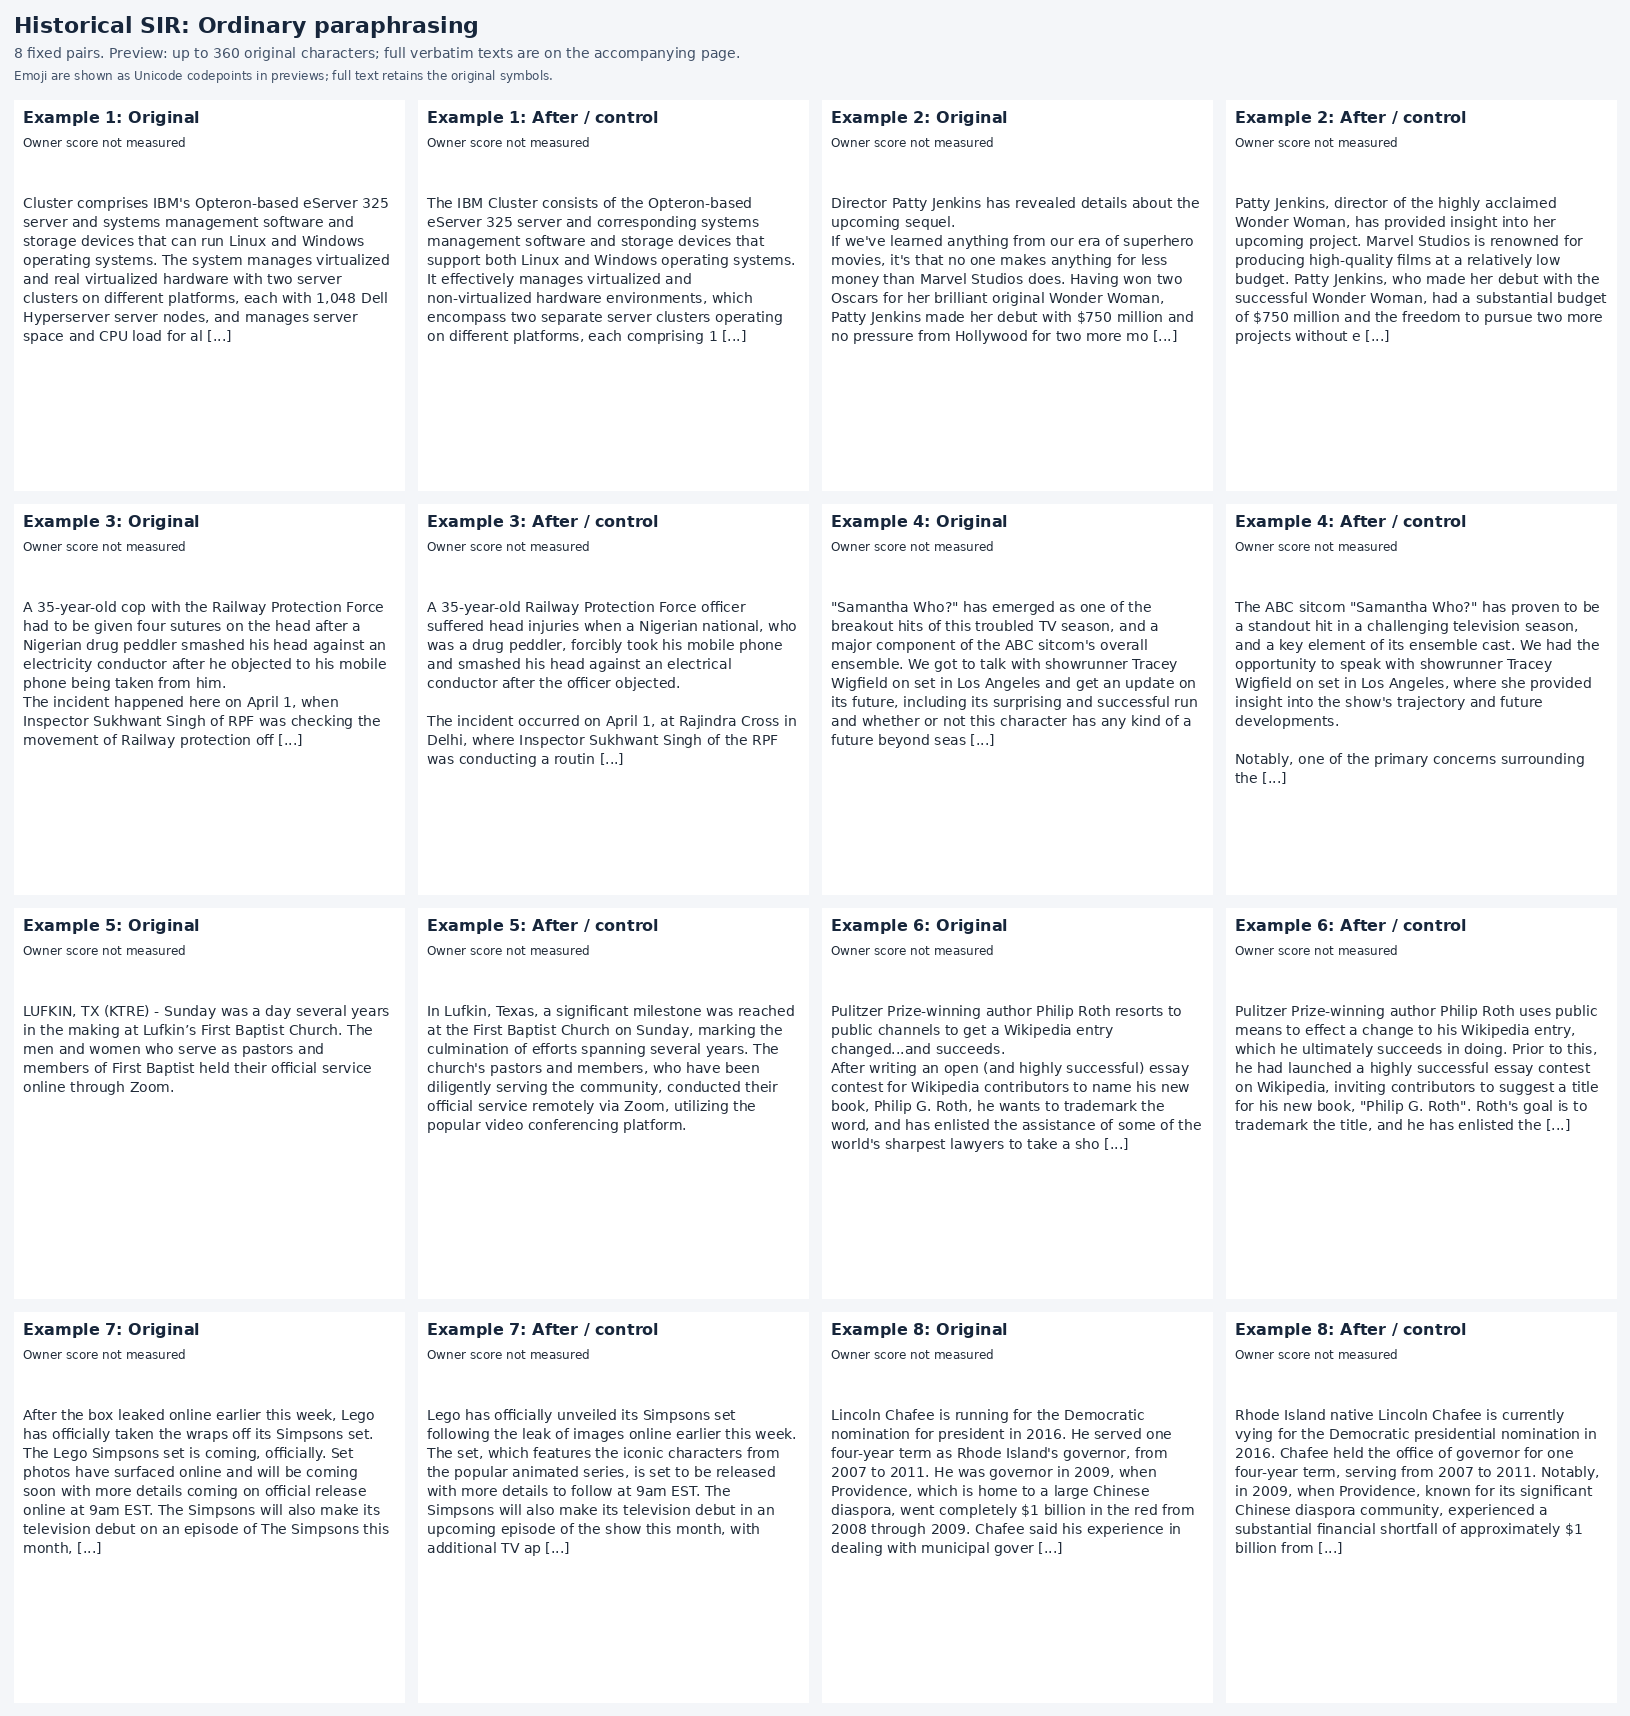
\includegraphics[keepaspectratio,alt={Sixteen-panel text preview}]{figures/paper-sir-vanilla.png}}
\caption{Sixteen-panel text preview}
\end{recordfigure}

The figure previews up to the first 360 original characters per
response; full texts below are unabridged. Emoji use Unicode codepoints
in the preview to avoid missing-glyph boxes. Owner scores and quality
metrics use full responses.

{\scriptsize\setlength{\tabcolsep}{3pt}\def\LTcaptype{none} % do not increment counter
\begin{longtable}[]{@{}
  >{\raggedright\arraybackslash}p{(\linewidth - 8\tabcolsep) * \real{0.2000}}
  >{\raggedright\arraybackslash}p{(\linewidth - 8\tabcolsep) * \real{0.2000}}
  >{\raggedright\arraybackslash}p{(\linewidth - 8\tabcolsep) * \real{0.2000}}
  >{\raggedright\arraybackslash}p{(\linewidth - 8\tabcolsep) * \real{0.2000}}
  >{\raggedright\arraybackslash}p{(\linewidth - 8\tabcolsep) * \real{0.2000}}@{}}
\toprule\noalign{}
\begin{minipage}[b]{\linewidth}\raggedright
Example
\end{minipage} & \begin{minipage}[b]{\linewidth}\raggedright
Test position
\end{minipage} & \begin{minipage}[b]{\linewidth}\raggedright
Before
\end{minipage} & \begin{minipage}[b]{\linewidth}\raggedright
After
\end{minipage} & \begin{minipage}[b]{\linewidth}\raggedright
Jina
\end{minipage} \\
\midrule\noalign{}
\endhead
\bottomrule\noalign{}
\endlastfoot
1 & 0 & Owner score not measured & Owner score not measured & not
measured \\
2 & 41 & Owner score not measured & Owner score not measured & not
measured \\
3 & 82 & Owner score not measured & Owner score not measured & not
measured \\
4 & 123 & Owner score not measured & Owner score not measured & not
measured \\
5 & 165 & Owner score not measured & Owner score not measured & not
measured \\
6 & 206 & Owner score not measured & Owner score not measured & not
measured \\
7 & 247 & Owner score not measured & Owner score not measured & not
measured \\
8 & 288 & Owner score not measured & Owner score not measured & not
measured \\
\end{longtable}
}

\subsection{Example 1: test position
0}\label{record-docs-watermarking-qualitative-paper-sir-vanilla-md-example-1-test-position-0}

Prompt ID:
\texttt{\seqsplit{e31e6f74ee79d4c901f4c7e2d71bc20b7d4ac16a960885a84dbed35ed994c04a}}.

\textbf{Question / prompt}

\begin{Verbatim}
Cluster comprises IBM's Opteron-based eServer 325 server and systems management software and storage devices that can run Linux and Windows operating systems
\end{Verbatim}

\textbf{Original watermarked-model output}

\begin{Verbatim}
Cluster comprises IBM's Opteron-based eServer 325 server and systems management software and storage devices that can run Linux and Windows operating systems. The system manages virtualized and real virtualized hardware with two server clusters on different platforms, each with 1,048 Dell Hyperserver server nodes, and manages server space and CPU load for all three clusters. Deployed in virtualized and remote distributed datacenters, and in the cloud, Clusters provide cloud and data center scalability along with improved availability and fault tolerance to allow for large-scale deployment of applications and virtual computing assets.

The eServer 325 system was developed to increase efficiency and scalability to satisfy the needs of cloud and datacenter developers.

"Our customers have been requesting virtualized and non-virtualized solutions for cloud and multi-node deployments from IBM for many products and we have seen tremendous market interest," said Bryan Murphy, senior program manager, Clusters at IBM Global Software. "Customers are increasingly looking at Clusters to provide increased capability, control and flexibility to satisfy their applications and data sets."

Availability and pricing of IBM Clusters are based on availability with an enterprise or shared server purchase, including 24-hour virtual machine capacity, as well as shared management, hardware, and
\end{Verbatim}

\textbf{After / alternative output}

\begin{Verbatim}
The IBM Cluster consists of the Opteron-based eServer 325 server and corresponding systems management software and storage devices that support both Linux and Windows operating systems. It effectively manages virtualized and non-virtualized hardware environments, which encompass two separate server clusters operating on different platforms, each comprising 1,048 Dell Hyperserver server nodes. This setup allows for the monitoring of server space and CPU load across all three clusters. Designed for deployment in virtualized and remote distributed data centers, as well as cloud environments, IBM Clusters offer enhanced scalability and improved availability and fault tolerance to facilitate large-scale applications and virtual computing asset deployment.

Developed to meet the demands of cloud and datacenter developers, the eServer 325 system is optimized for increased efficiency and scalability. According to Bryan Murphy, senior program manager for Clusters at IBM Global Software, customer demand for virtualized and non-virtualized solutions for cloud and multi-node deployments has been significant, with substantial market interest. As a result, customers are increasingly turning to IBM Clusters to provide enhanced capabilities, control, and flexibility to meet their application and data set requirements.

IBM Clusters' availability and pricing are tied to enterprise or shared server purchases, which include 24-hour virtual machine capacity, as well as shared management, hardware, and other resources.
\end{Verbatim}

\subsection{Example 2: test position
41}\label{record-docs-watermarking-qualitative-paper-sir-vanilla-md-example-2-test-position-41}

Prompt ID:
\texttt{\seqsplit{f349a8727c7c51a1c91fedf1fcafe0ae6851c5474bb2ce79fccc84c7544358e8}}.

\textbf{Question / prompt}

\begin{Verbatim}
Director Patty Jenkins has revealed details about the upcoming sequel.
If we've learned anything from our era of superhero movies, it's that no one
\end{Verbatim}

\textbf{Original watermarked-model output}

\begin{Verbatim}
Director Patty Jenkins has revealed details about the upcoming sequel.
If we've learned anything from our era of superhero movies, it's that no one makes anything for less money than Marvel Studios does. Having won two Oscars for her brilliant original Wonder Woman, Patty Jenkins made her debut with $750 million and no pressure from Hollywood for two more movies. The good news for a woman who's never seen any comic book characters and not entirely sure if she wants to even, Wonder Woman 1984 wasn't her first foray into comic books, having previously worked with Marc Webb on the highly successful Daredevil and Jessica Jones, with both not being good movies, or movies with any female leads to be frank, and it turned into $790,070,000 at the box office and went on to win an Oscar in its own right for its visual story telling.
When asked if she knows anything about her future in the comic book world, Patty Jenkins has said that not really and if she does want to come back, that she'll certainly be doing her damndest to make her vision known. She has also revealed an interesting bit of information though, saying that she plans her movies with female characters at her heart, and won't be making something for men. Checkout an excerpt from her comments below,
\end{Verbatim}

\textbf{After / alternative output}

\begin{Verbatim}
Patty Jenkins, director of the highly acclaimed Wonder Woman, has provided insight into her upcoming project. Marvel Studios is renowned for producing high-quality films at a relatively low budget. Patty Jenkins, who made her debut with the successful Wonder Woman, had a substantial budget of $750 million and the freedom to pursue two more projects without external pressure. This financial independence is a rare commodity in Hollywood.

Interestingly, Patty Jenkins' foray into comic book films began before her work on Wonder Woman 1984. She collaborated with Marc Webb on the TV series Daredevil and Jessica Jones, although it's worth noting that these projects received mixed reviews. Nevertheless, Wonder Woman 1984 achieved significant box office success, grossing $790,070,000 and earning an Oscar for its visual storytelling.

When asked about her potential future in the comic book world, Patty Jenkins expressed uncertainty, stating that she doesn't have any concrete plans. However, if she were to return, she would strive to maintain creative control. Notably, Patty Jenkins has revealed that she prioritizes films centered around female characters, indicating that her future projects will likely focus on this aspect. In her own words, she intends to create movies that cater to female audiences and avoid catering exclusively to male viewers.
\end{Verbatim}

\subsection{Example 3: test position
82}\label{record-docs-watermarking-qualitative-paper-sir-vanilla-md-example-3-test-position-82}

Prompt ID:
\texttt{\seqsplit{a8aa4f7effda3b9a9f5d3ee789d1d3c1dcb65a4df31ca926e955d1241abda5e1}}.

\textbf{Question / prompt}

\begin{Verbatim}
A 35-year-old cop with the Railway Protection Force had to be given four sutures on the head after a Nigerian drug peddler
\end{Verbatim}

\textbf{Original watermarked-model output}

\begin{Verbatim}
A 35-year-old cop with the Railway Protection Force had to be given four sutures on the head after a Nigerian drug peddler smashed his head against an electricity conductor after he objected to his mobile phone being taken from him.
The incident happened here on April 1, when Inspector Sukhwant Singh of RPF was checking the movement of Railway protection officers at Rajindra Cross in Delhi when Doremus Abdada, 32, of Odisha, tried to take his mobile phone. Inspector Sukhwait tried to take the mobile phone from him and started telling him to allow them to take him through security.
The accused, however, smashed one of the policeman’s forehead and claimed he could not hear. As he couldn’t distinguish between words and sounds, Inspector Sukhshit Singh asked him to give a physical description. Mr. Doremus, however, said he could not give one.
The Inspector, said Senior Executive Magistrate Dharmendra Nath Singh, said, he had a problem imagining that he himself had been injured. Constable Manoj, a resident of Malviya Nagar, was driving Inspector Sukhwit Singh’s vehicle.
The police said they were patrolling Rajindra Crossing when they received a PCR call
\end{Verbatim}

\textbf{After / alternative output}

\begin{Verbatim}
A 35-year-old Railway Protection Force officer suffered head injuries when a Nigerian national, who was a drug peddler, forcibly took his mobile phone and smashed his head against an electrical conductor after the officer objected.

The incident occurred on April 1, at Rajindra Cross in Delhi, where Inspector Sukhwant Singh of the RPF was conducting a routine check on Railway protection officers. During this operation, Doremus Abdada, a 32-year-old from Odisha, attempted to take the inspector's mobile phone. Inspector Sukhwant Singh intervened and instructed Doremus to allow himself to be taken through security checks.

However, Doremus responded by violently smashing his forehead against the inspector's head. Despite his actions, Doremus claimed he couldn't hear the inspector. Due to his inability to distinguish between words and sounds, Inspector Sukhwant Singh requested a physical description from Doremus. Nonetheless, Doremus stated that he was unable to provide one.

According to Senior Executive Magistrate Dharmendra Nath Singh, the inspector had difficulty comprehending that he himself had been injured. Meanwhile, Constable Manoj, a resident of Malviya Nagar, was driving the vehicle belonging to Inspector Sukhwant Singh at the time of the incident. The police were patrolling Rajindra Crossing when they received a PCR call.
\end{Verbatim}

\subsection{Example 4: test position
123}\label{record-docs-watermarking-qualitative-paper-sir-vanilla-md-example-4-test-position-123}

Prompt ID:
\texttt{\seqsplit{adaf979fdfb964904e387f40af11efc473f86dfd03a188d448f24221cea6cf05}}.

\textbf{Question / prompt}

\begin{Verbatim}
"Samantha Who?" has emerged as one of the breakout hits of this troubled TV season, and a major component of the ABC sitcom's
\end{Verbatim}

\textbf{Original watermarked-model output}

\begin{Verbatim}
"Samantha Who?" has emerged as one of the breakout hits of this troubled TV season, and a major component of the ABC sitcom's overall ensemble. We got to talk with showrunner Tracey Wigfield on set in Los Angeles and get an update on its future, including its surprising and successful run and whether or not this character has any kind of a future beyond season two and its finale in March 2012...

Now, the question arises... how will Samantha take over her father's house in season three, how will Sam (ahem) and Samantha interact with her new friends [U+2014] and not to mention, how will Samantha be able to keep up her relationship with her ex Chris (ahem, Chris B.) and her mom? As Wigfield explains, "Samantha takes over from father Bob (David Farr) in season three." And not just any old season, but three, not including the original [U+2014] or original and two later [U+2014] airing Season One and its infamous cliffhanger, even if Samantha does take over.

When asked to predict when Samantha takes over, Wigfield offers, "I don't want to be too specific." She also wants to let us know something [U+2014] in regard to her character Samantha, who will apparently be
\end{Verbatim}

\textbf{After / alternative output}

\begin{Verbatim}
The ABC sitcom "Samantha Who?" has proven to be a standout hit in a challenging television season, and a key element of its ensemble cast. We had the opportunity to speak with showrunner Tracey Wigfield on set in Los Angeles, where she provided insight into the show's trajectory and future developments. 

Notably, one of the primary concerns surrounding the series revolves around Samantha's future beyond season two, particularly in relation to her inheritance of her father's house in season three. Additionally, there are questions surrounding Samantha's relationships with her new acquaintances and her ex Chris (Chris B.), as well as her interactions with her mother. Wigfield clarified that "Samantha takes over from father Bob (David Farr) in season three," which will mark a significant milestone for the character.

When asked for a more specific timeline for Samantha's takeover, Wigfield opted to exercise caution, stating, "I don't want to be too specific." Nonetheless, she chose to share that the show will continue to unfold, with Samantha navigating her relationships and new circumstances.
\end{Verbatim}

\subsection{Example 5: test position
165}\label{record-docs-watermarking-qualitative-paper-sir-vanilla-md-example-5-test-position-165}

Prompt ID:
\texttt{\seqsplit{1b3ba6e9a2d857aa37a67122f763b84f6e273823246f7c6fcec9fced3d89d443}}.

\textbf{Question / prompt}

\begin{Verbatim}
LUFKIN, TX (KTRE) - Sunday was a day several years in the making at Lufkin’s First Baptist Church
\end{Verbatim}

\textbf{Original watermarked-model output}

\begin{Verbatim}
LUFKIN, TX (KTRE) - Sunday was a day several years in the making at Lufkin’s First Baptist Church. The men and women who serve as pastors and members of First Baptist held their official service online through Zoom.
\end{Verbatim}

\textbf{After / alternative output}

\begin{Verbatim}
In Lufkin, Texas, a significant milestone was reached at the First Baptist Church on Sunday, marking the culmination of efforts spanning several years. The church's pastors and members, who have been diligently serving the community, conducted their official service remotely via Zoom, utilizing the popular video conferencing platform.
\end{Verbatim}

\subsection{Example 6: test position
206}\label{record-docs-watermarking-qualitative-paper-sir-vanilla-md-example-6-test-position-206}

Prompt ID:
\texttt{\seqsplit{03347445733f407fb1ccdcdfee0ac8a6870be235b90c64510ee96dfa7af4dfcf}}.

\textbf{Question / prompt}

\begin{Verbatim}
Pulitzer Prize-winning author Philip Roth resorts to public channels to get a Wikipedia entry changed...and succeeds.
After writing an open (
\end{Verbatim}

\textbf{Original watermarked-model output}

\begin{Verbatim}
Pulitzer Prize-winning author Philip Roth resorts to public channels to get a Wikipedia entry changed...and succeeds.
After writing an open (and highly successful) essay contest for Wikipedia contributors to name his new book, Philip G. Roth, he wants to trademark the word, and has enlisted the assistance of some of the world's sharpest lawyers to take a shot at gaining control of its use in print and in the electronic medium. But just when he thinks he's got his ducks in a row, his project has its first, and big, problem. So how can he win back support from not only Wikipedia, but also from his legions of fans, many of whom have rallied around the challenge he laid on them, and from his former publisher, Houghton Mifflin Harcourt, where he has been editor since he departed from his previous editor, Neal Gabler, in 2012, after Gabler left to work at Penguin Group. We talk with Philip. [U+2014] Adam Clark
\end{Verbatim}

\textbf{After / alternative output}

\begin{Verbatim}
Pulitzer Prize-winning author Philip Roth uses public means to effect a change to his Wikipedia entry, which he ultimately succeeds in doing. Prior to this, he had launched a highly successful essay contest on Wikipedia, inviting contributors to suggest a title for his new book, "Philip G. Roth". Roth's goal is to trademark the title, and he has enlisted the help of top lawyers to attempt to secure exclusive rights to its use in both print and digital formats. However, just as Roth thought he was making progress, his project encountered its first major obstacle. In light of this setback, Roth must find a way to regain the support of not only Wikipedia, but also his devoted fan base, which had rallied behind the challenge he presented, as well as his former publisher, Houghton Mifflin Harcourt, where he has been working since his departure from his previous editor, Neal Gabler, in 2012. Neal Gabler had left his position at Houghton Mifflin Harcourt to join Penguin Group at that time. We spoke with Philip Roth about this development.
\end{Verbatim}

\subsection{Example 7: test position
247}\label{record-docs-watermarking-qualitative-paper-sir-vanilla-md-example-7-test-position-247}

Prompt ID:
\texttt{\seqsplit{4cbf4e262824ea813199d26415d873e7a935d3d4f9e628144b1679a9ef93d63a}}.

\textbf{Question / prompt}

\begin{Verbatim}
After the box leaked online earlier this week, Lego has officially taken the wraps off its Simpsons set.
The Lego Simpsons set is coming, officially
\end{Verbatim}

\textbf{Original watermarked-model output}

\begin{Verbatim}
After the box leaked online earlier this week, Lego has officially taken the wraps off its Simpsons set.
The Lego Simpsons set is coming, officially. Set photos have surfaced online and will be coming soon with more details coming on official release online at 9am EST. The Simpsons will also make its television debut on an episode of The Simpsons this month, and will be making more TV appearances in 2019. But in preparation for these new appearances, the Simpsons creator Matt Groening has hinted at some Simpsons characters making appearances in movies soon, too. Check out previous Simpsons appearances in movies here and here, and see how he says it could play into movies here.
It's not the Simpsons you're looking for, but it could be something else! The Simpsons: The Movie will be in theaters in 2019 and while details are thin at this point, perhaps we'll get to see some other characters from the past make an appearance, or have some familiar characters make an unexpected appearance. So perhaps we'll see Uncle Moe from Happy Days, who would be fun to have. Or maybe we'll just get to see an old friend and maybe see The Chief Marge again, though we don't think he has an age limit. He could be in his 90s, if his voice has remained intact,
\end{Verbatim}

\textbf{After / alternative output}

\begin{Verbatim}
Lego has officially unveiled its Simpsons set following the leak of images online earlier this week. The set, which features the iconic characters from the popular animated series, is set to be released with more details to follow at 9am EST. The Simpsons will also make its television debut in an upcoming episode of the show this month, with additional TV appearances planned for 2019. In anticipation of these new appearances, creator Matt Groening has hinted that some Simpsons characters may also be featured in movies in the near future. For reference, previous Simpsons movie appearances can be viewed here and here, and Groening's comments on the potential for movie involvement can be seen here.

It appears that this is not the Simpsons movie that fans are expecting. Instead, The Simpsons: The Movie is scheduled for release in 2019, although details are currently scarce. It is possible that the movie may feature appearances by characters from the past or unexpected cameos from familiar faces. Some potential possibilities include Uncle Moe from Happy Days or a return by Chief Wiggum, who, despite his advanced age, could potentially make an appearance if his voice remains intact.
\end{Verbatim}

\subsection{Example 8: test position
288}\label{record-docs-watermarking-qualitative-paper-sir-vanilla-md-example-8-test-position-288}

Prompt ID:
\texttt{\seqsplit{9cdf452ec7392837b8e59d71537c6bd8a5a860e4379361d145f1b68dc8ef065b}}.

\textbf{Question / prompt}

\begin{Verbatim}
Lincoln Chafee is running for the Democratic nomination for president in 2016. He served one four-year term as Rhode Island's governor,
\end{Verbatim}

\textbf{Original watermarked-model output}

\begin{Verbatim}
Lincoln Chafee is running for the Democratic nomination for president in 2016. He served one four-year term as Rhode Island's governor, from 2007 to 2011. He was governor in 2009, when Providence, which is home to a large Chinese diaspora, went completely $1 billion in the red from 2008 through 2009. Chafee said his experience in dealing with municipal governments and state budgets in Rhode Island made him an ideal candidate to represent Rhode Island in D.C.

Toby Ann Curry, the host of NPR's The Place to Be, returned to her hometown to share her two new books, The Place She Ate and The Place She Sang, and to talk about writing and her work with TED. From The New Yorker magazine, here are quotes from three authors and authors-to-be who spoke from and around NPR's studios: Chafee, Curry and her mother, Nobel Peace Prize laureate Malala Yousafzai.

Author Sarah Duhatschek has been featured in The Boston Globe, The New York Times and The Boston Herald, among a dozen other national and international publications for her book, The Last Mile: An Essay On Sports, Family, And Happiness On The Last Mile That Fails And Fails And Gets
\end{Verbatim}

\textbf{After / alternative output}

\begin{Verbatim}
Rhode Island native Lincoln Chafee is currently vying for the Democratic presidential nomination in 2016. Chafee held the office of governor for one four-year term, serving from 2007 to 2011. Notably, in 2009, when Providence, known for its significant Chinese diaspora community, experienced a substantial financial shortfall of approximately $1 billion from 2008 through 2009. Chafee cited his experience managing municipal governments and state budgets in Rhode Island as a key qualification for representing the state in Washington D.C.

Toby Ann Curry, the host of NPR's The Place to Be, returned to her hometown to discuss her recent publications, The Place She Ate and The Place She Sang, as well as her work with TED. The following quotes come from a gathering of authors and aspiring writers at NPR's studios, featuring Chafee, Curry, and her mother, Malala Yousafzai, a renowned Nobel Peace Prize laureate.
\end{Verbatim}

\href{records/docs/watermarking/text.tex}{Text metrics} \textbar{}
\href{../docs/watermarking/README.md}{Report overview}
